\documentclass[svgnames, 12pt]{beamer}

%----------------------------------------------------------------------------------------
%   PACKAGES AND THEMES
%----------------------------------------------------------------------------------------

\usepackage[utf8]{inputenc}
\usepackage[english]{babel}
\usepackage[L7x]{fontenc}
\usepackage{lmodern}
\usepackage{amsmath}
\usepackage{amssymb}
\usepackage{xcolor}
\usepackage{subfig}
\usepackage{graphicx}
\usepackage{lipsum}
\usepackage{hyperref}

\definecolor{mifcolor}{RGB}{0, 71, 127}
\definecolor{dimgr}{RGB}{105, 105, 105}
\definecolor{sky}{RGB}{0, 191, 255}
\setbeamercolor{alerted text}{fg=red,bg=sky}
\newcommand{\boxalert}[1]{{%
	\usebeamercolor{alerted text}\colorbox{bg}{\alert{#1}}%
}}

\mode<presentation>{
	\usetheme{Madrid}
	\usecolortheme[named=mifcolor]{structure}
	\setbeamertemplate{footline}
	{%
		\leavevmode%
		\hbox{
			\begin{beamercolorbox}[wd=.3\paperwidth,ht=2.5ex,dp=1.125ex,leftskip=.3cm
				plus1fill,rightskip=.3cm]{author in head/foot}%
				\usebeamerfont{author in head/foot}\insertshortauthor \hfill
			\end{beamercolorbox}%
			\begin{beamercolorbox}[wd=.2\paperwidth,ht=2.5ex,dp=1.125ex,leftskip=.3cm,
				rightskip=.3cm plus1fil]{institute in head/foot}%
				\usebeamerfont{institute in head/foot}\insertshortinstitute
			\end{beamercolorbox}%
			\begin{beamercolorbox}[wd=.2\paperwidth,ht=2.5ex,dp=1.125ex,leftskip=.3cm,
				rightskip=.3cm plus1fil]{date in head/foot}%
				\usebeamerfont{date in head/foot}\insertshortdate
			\end{beamercolorbox}%
			\begin{beamercolorbox}[wd=.3\paperwidth,ht=2.5ex,dp=1.125ex,leftskip=.3cm,
				rightskip=.3cm plus1fil]{title in head/foot}%
				\usebeamerfont{title in head/foot}\insertshorttitle\hfill p.
				\insertframenumber\enspace of \inserttotalframenumber\enspace 
			\end{beamercolorbox}
		}%
		\vskip0pt%
	}
}

\title[Air Quality Analysis in Delhi]{Multivariate Time Series Analysis of Air Quality Data in Delhi}
\author[A. J. Smoliakov]{Aleksandr Jan Smoliakov\inst{1}}
\institute[VU MIF]{\inst{1} Vilnius University, Faculty of Mathematics and Informatics}
\date{2025--05--27}

%----------------------------------------------------------------------------------------
%   BEGIN DOCUMENT
%----------------------------------------------------------------------------------------
\begin{document}

%----------------------------------------------------------------------------------------
%   TITLE FRAME
%----------------------------------------------------------------------------------------
\begin{frame}
	
\includegraphics[scale=0.15]{MIF Garamond-logo.png} 
	\hfill
	
\includegraphics[scale=0.15]{Logo_spalvotas.eps}
	\titlepage
\end{frame}

%----------------------------------------------------------------------------------------
%   TABLE OF CONTENTS FRAME
%----------------------------------------------------------------------------------------
\begin{frame}{Table of Contents}
\tableofcontents
\end{frame}

%----------------------------------------------------------------------------------------
\section{Introduction}
%----------------------------------------------------------------------------------------
\begin{frame}
    \frametitle{Introduction: The Air Quality Challenge}
    \begin{itemize}
        \item Urban air quality is a critical public health and environmental issue, especially in rapidly urbanizing regions like Delhi.
        \item Accurate forecasting of pollutants (e.g., $PM_{2.5}$, $PM_{10}$, $NO_2$, CO) is essential for timely policy interventions.
        \item Univariate models (e.g., ARIMA) offer a baseline but may not capture complex interdependencies.
        \item Multivariate time series models (e.g., VAR, VARMA), prominent in financial econometrics, can model interactions between multiple pollutant series.
    \end{itemize}
    \vspace{0.5cm}
    \begin{block}{Focus of this Project}
        Analyze air quality in Delhi (2018-2019) using daily data for five key pollutants: $PM_{2.5}$, $PM_{10}$, $NO_2$, CO, and $NH_3$.
    \end{block}
\end{frame}

%----------------------------------------------------------------------------------------
\begin{frame}
    \frametitle{Project Objectives}
    \begin{itemize}
        \item To apply multivariate time series models (VAR and VARMA) to understand the dynamic interactions among key air pollutants in Delhi.
        \item To generate forecasts for these pollutant concentrations.
        \item Key steps involved:
        \begin{itemize}
            \item Data preprocessing and Exploratory Data Analysis (EDA).
            \item Stationarity testing.
            \item VAR and VARMA model estimation and diagnostics.
            \item Granger causality analysis.
            \item Impulse Response Function (IRF) analysis.
            \item Forecast Error Variance Decomposition (FEVD).
            \item Forecast evaluation.
        \end{itemize}
    \end{itemize}
\end{frame}

%----------------------------------------------------------------------------------------
\section{Literature Snapshot}
%----------------------------------------------------------------------------------------
\begin{frame}
    \frametitle{Brief Literature Review}
    \begin{itemize}
        \item \textbf{Sethi and Mittal (2020):} Compared ARIMA and VAR for AQI in Gurugram. Found ARIMA more accurate, highlighting challenges with VAR stability and noise in interdependent series.
        \item \textbf{Hajmohammadi and Heydecker (2021):} Compared SARMA and VARMA for London air quality. VARMA outperformed by capturing cross-station interactions, emphasizing spatial dependency benefits.
        \item \textbf{Aladağ (2021):} Proposed a hybrid ARIMA model with wavelet transformation and seasonal adjustment for PM10 forecasting, addressing nonstationarity and seasonality.
    \end{itemize}
    \vspace{0.5cm}
    \begin{alertblock}{Key Takeaway}
        Multivariate frameworks are promising. Adapting techniques from fields like finance and using advanced data transformations can enhance model performance for environmental data.
    \end{alertblock}
\end{frame}

%----------------------------------------------------------------------------------------
\section{Methodology}
%----------------------------------------------------------------------------------------
\begin{frame}
    \frametitle{Data Source and Preparation}
    \begin{itemize}
        \item \textbf{Dataset:} \textit{Air Quality Data in India (2015--2020)}.
        \item \textbf{Focus:} Delhi, Jan 1, 2018 -- Jan 1, 2020 (732 daily observations).
        \item \textbf{Pollutants:} $PM_{2.5}$, $PM_{10}$, $NO_2$, CO, $NH_3$.
        \item \textbf{Reasons for Delhi focus:}
            \begin{itemize}
                \item One of the world's most polluted cities.
                \item Relatively complete data ($<1\%$ missing values for the selected period).
            \end{itemize}
        \item \textbf{Missing Value Imputation:} Linear interpolation (\texttt{na.interp}).
        \item \textbf{Data Transformation:} $\log(x+1)$ (log1p) to stabilize variance and normalize distributions.
        \item \textbf{Data Aggregation:} Hourly data aggregated to daily means (of log1p-transformed values) to reduce noise.
    \end{itemize}
\end{frame}

%----------------------------------------------------------------------------------------
\begin{frame}
    \frametitle{Exploratory Data Analysis (EDA)}
    \begin{itemize}
        \item \textbf{Distributions after transformation:}
    \end{itemize}
    \begin{figure}
        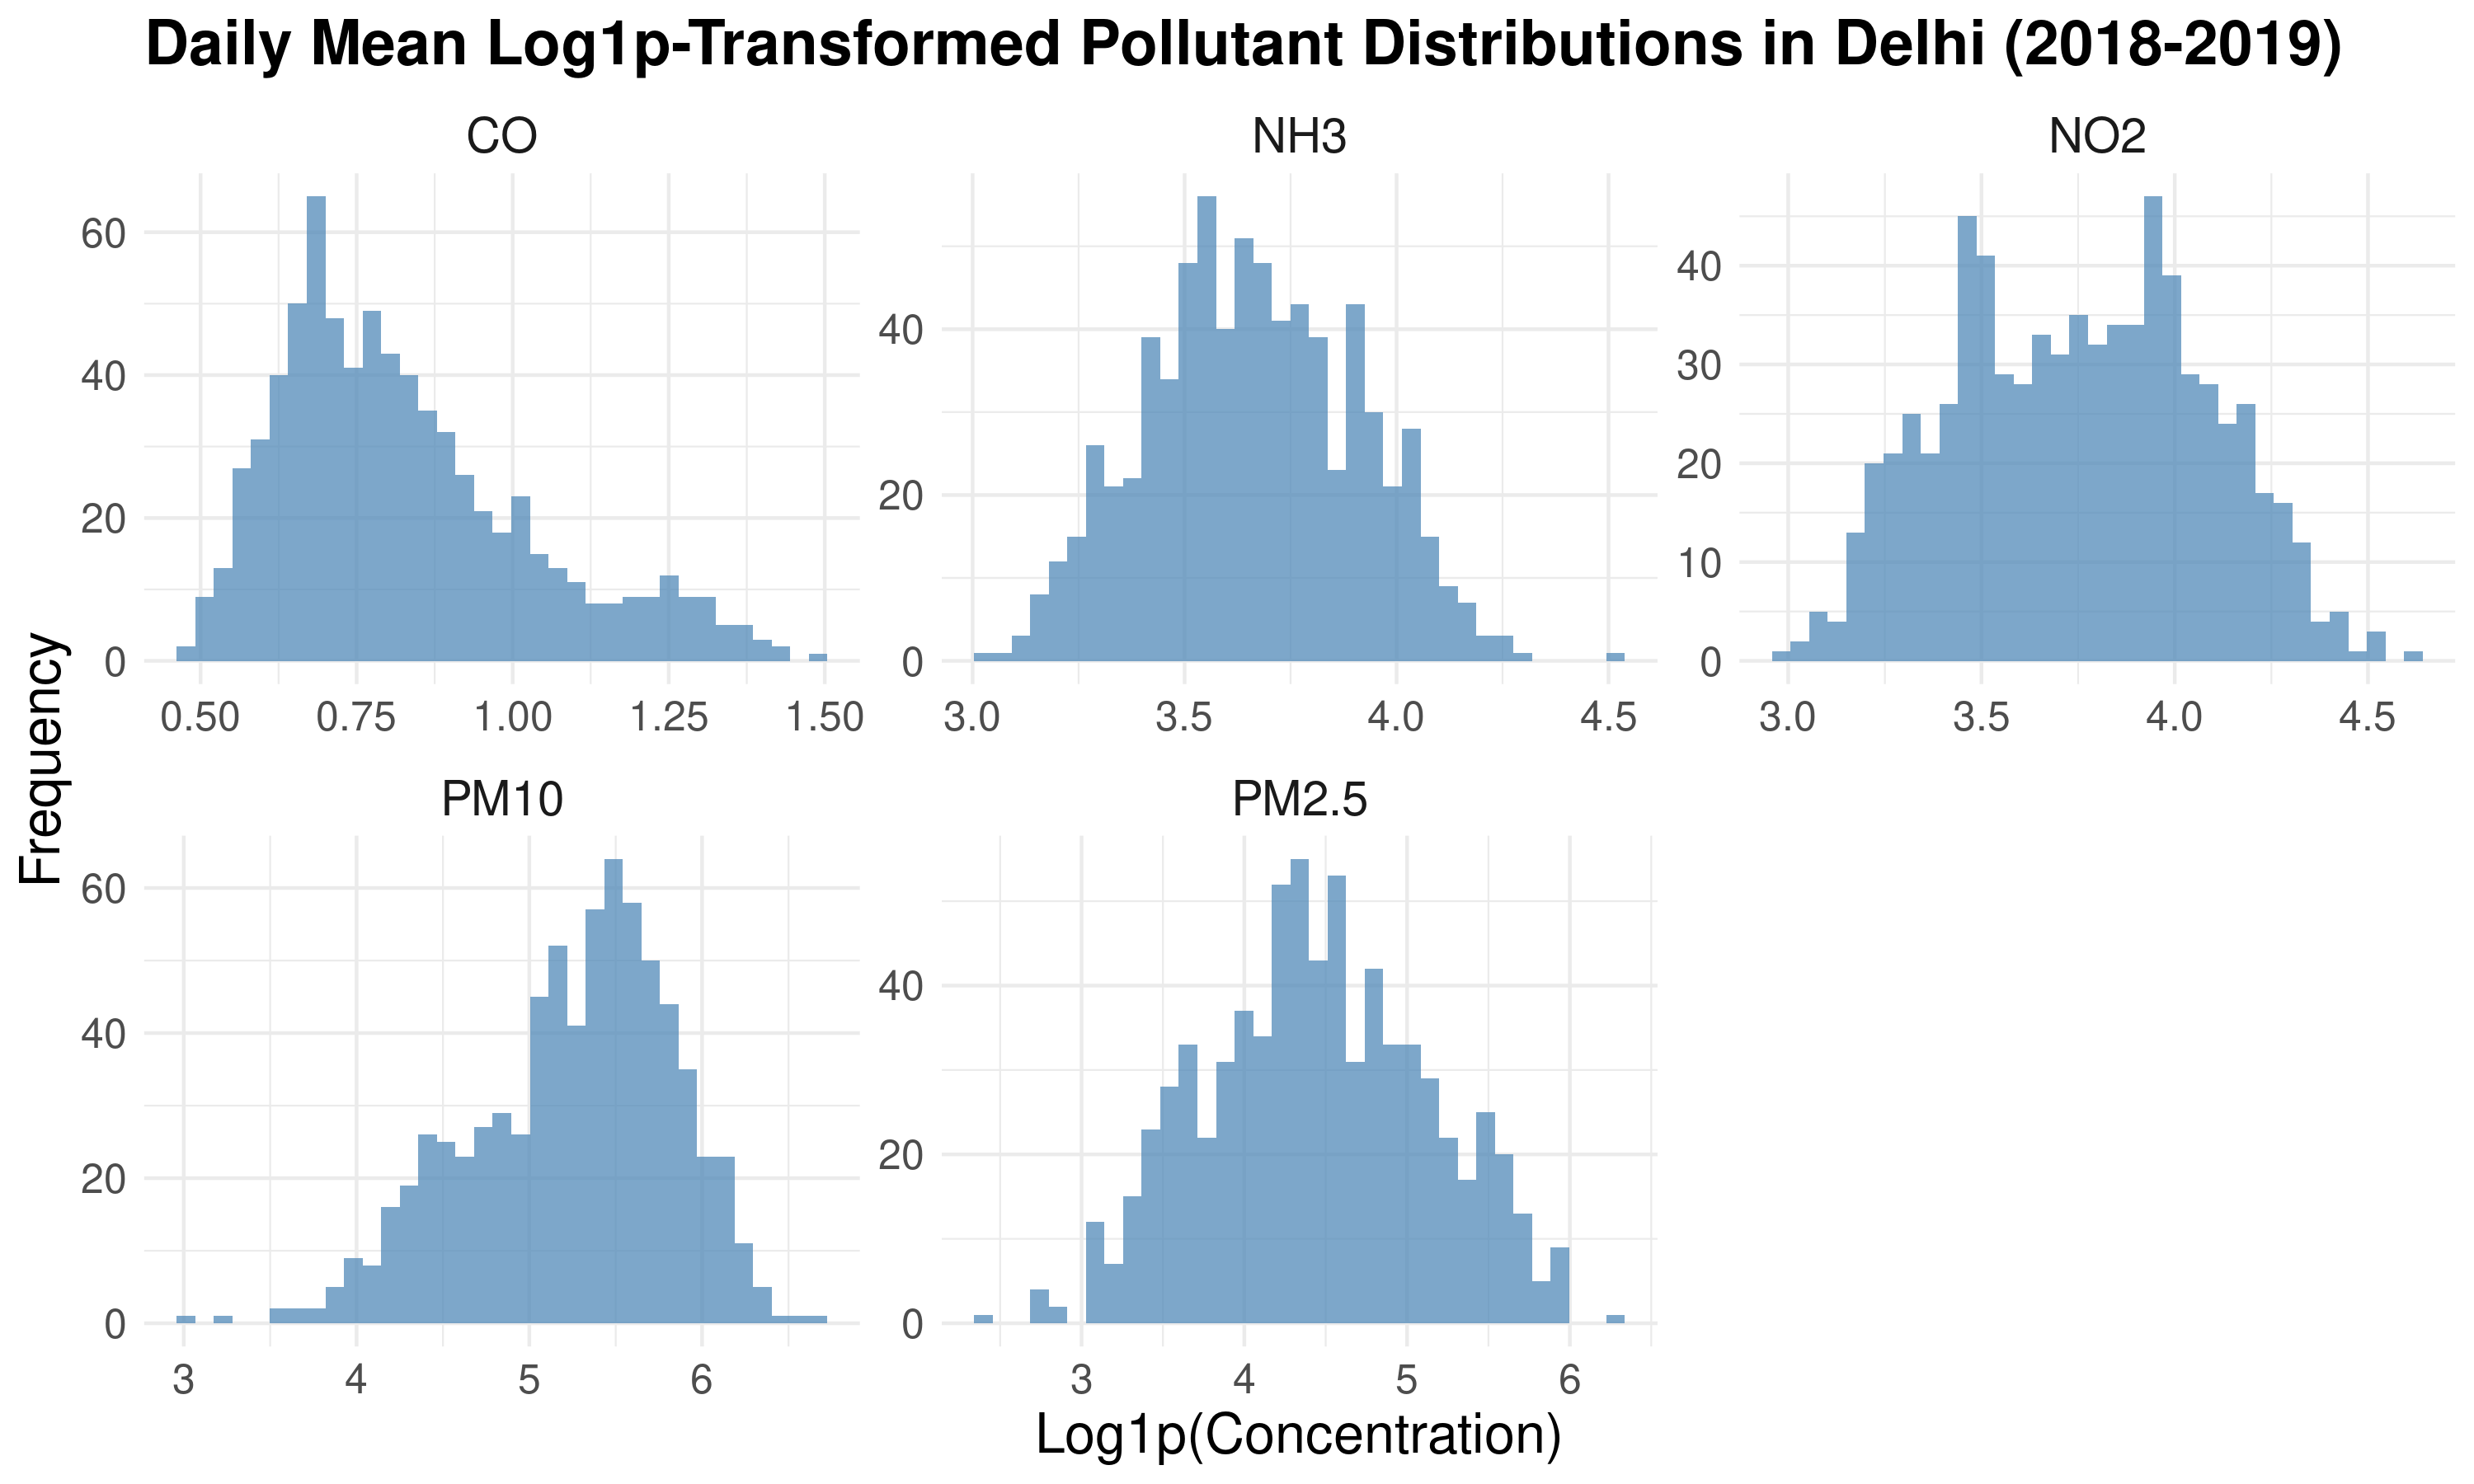
\includegraphics[width=0.8\linewidth]{../analysis/assets/log1p_delhi_distributions.png}
        \caption{Histograms of Daily Mean log1p-Transformed Pollutants (Delhi, 2018-2019).}
        \label{fig:log_dist_delhi_pres}
    \end{figure}
    \begin{itemize}
        \item Time series plots showed seasonality (higher pollution in winter).
        \item Correlation matrix revealed strong positive correlations (e.g., $PM_{2.5}$ \& $PM_{10}$: 0.93; $NO_2$ \& CO: 0.86).
    \end{itemize}
\end{frame}

%----------------------------------------------------------------------------------------
\begin{frame}
    \frametitle{EDA: Time Series and Correlations}
    \begin{columns}[T] % Split slide into two columns
        \begin{column}{0.5\textwidth}
            \textbf{Time Series Behavior:}
            \begin{figure}
                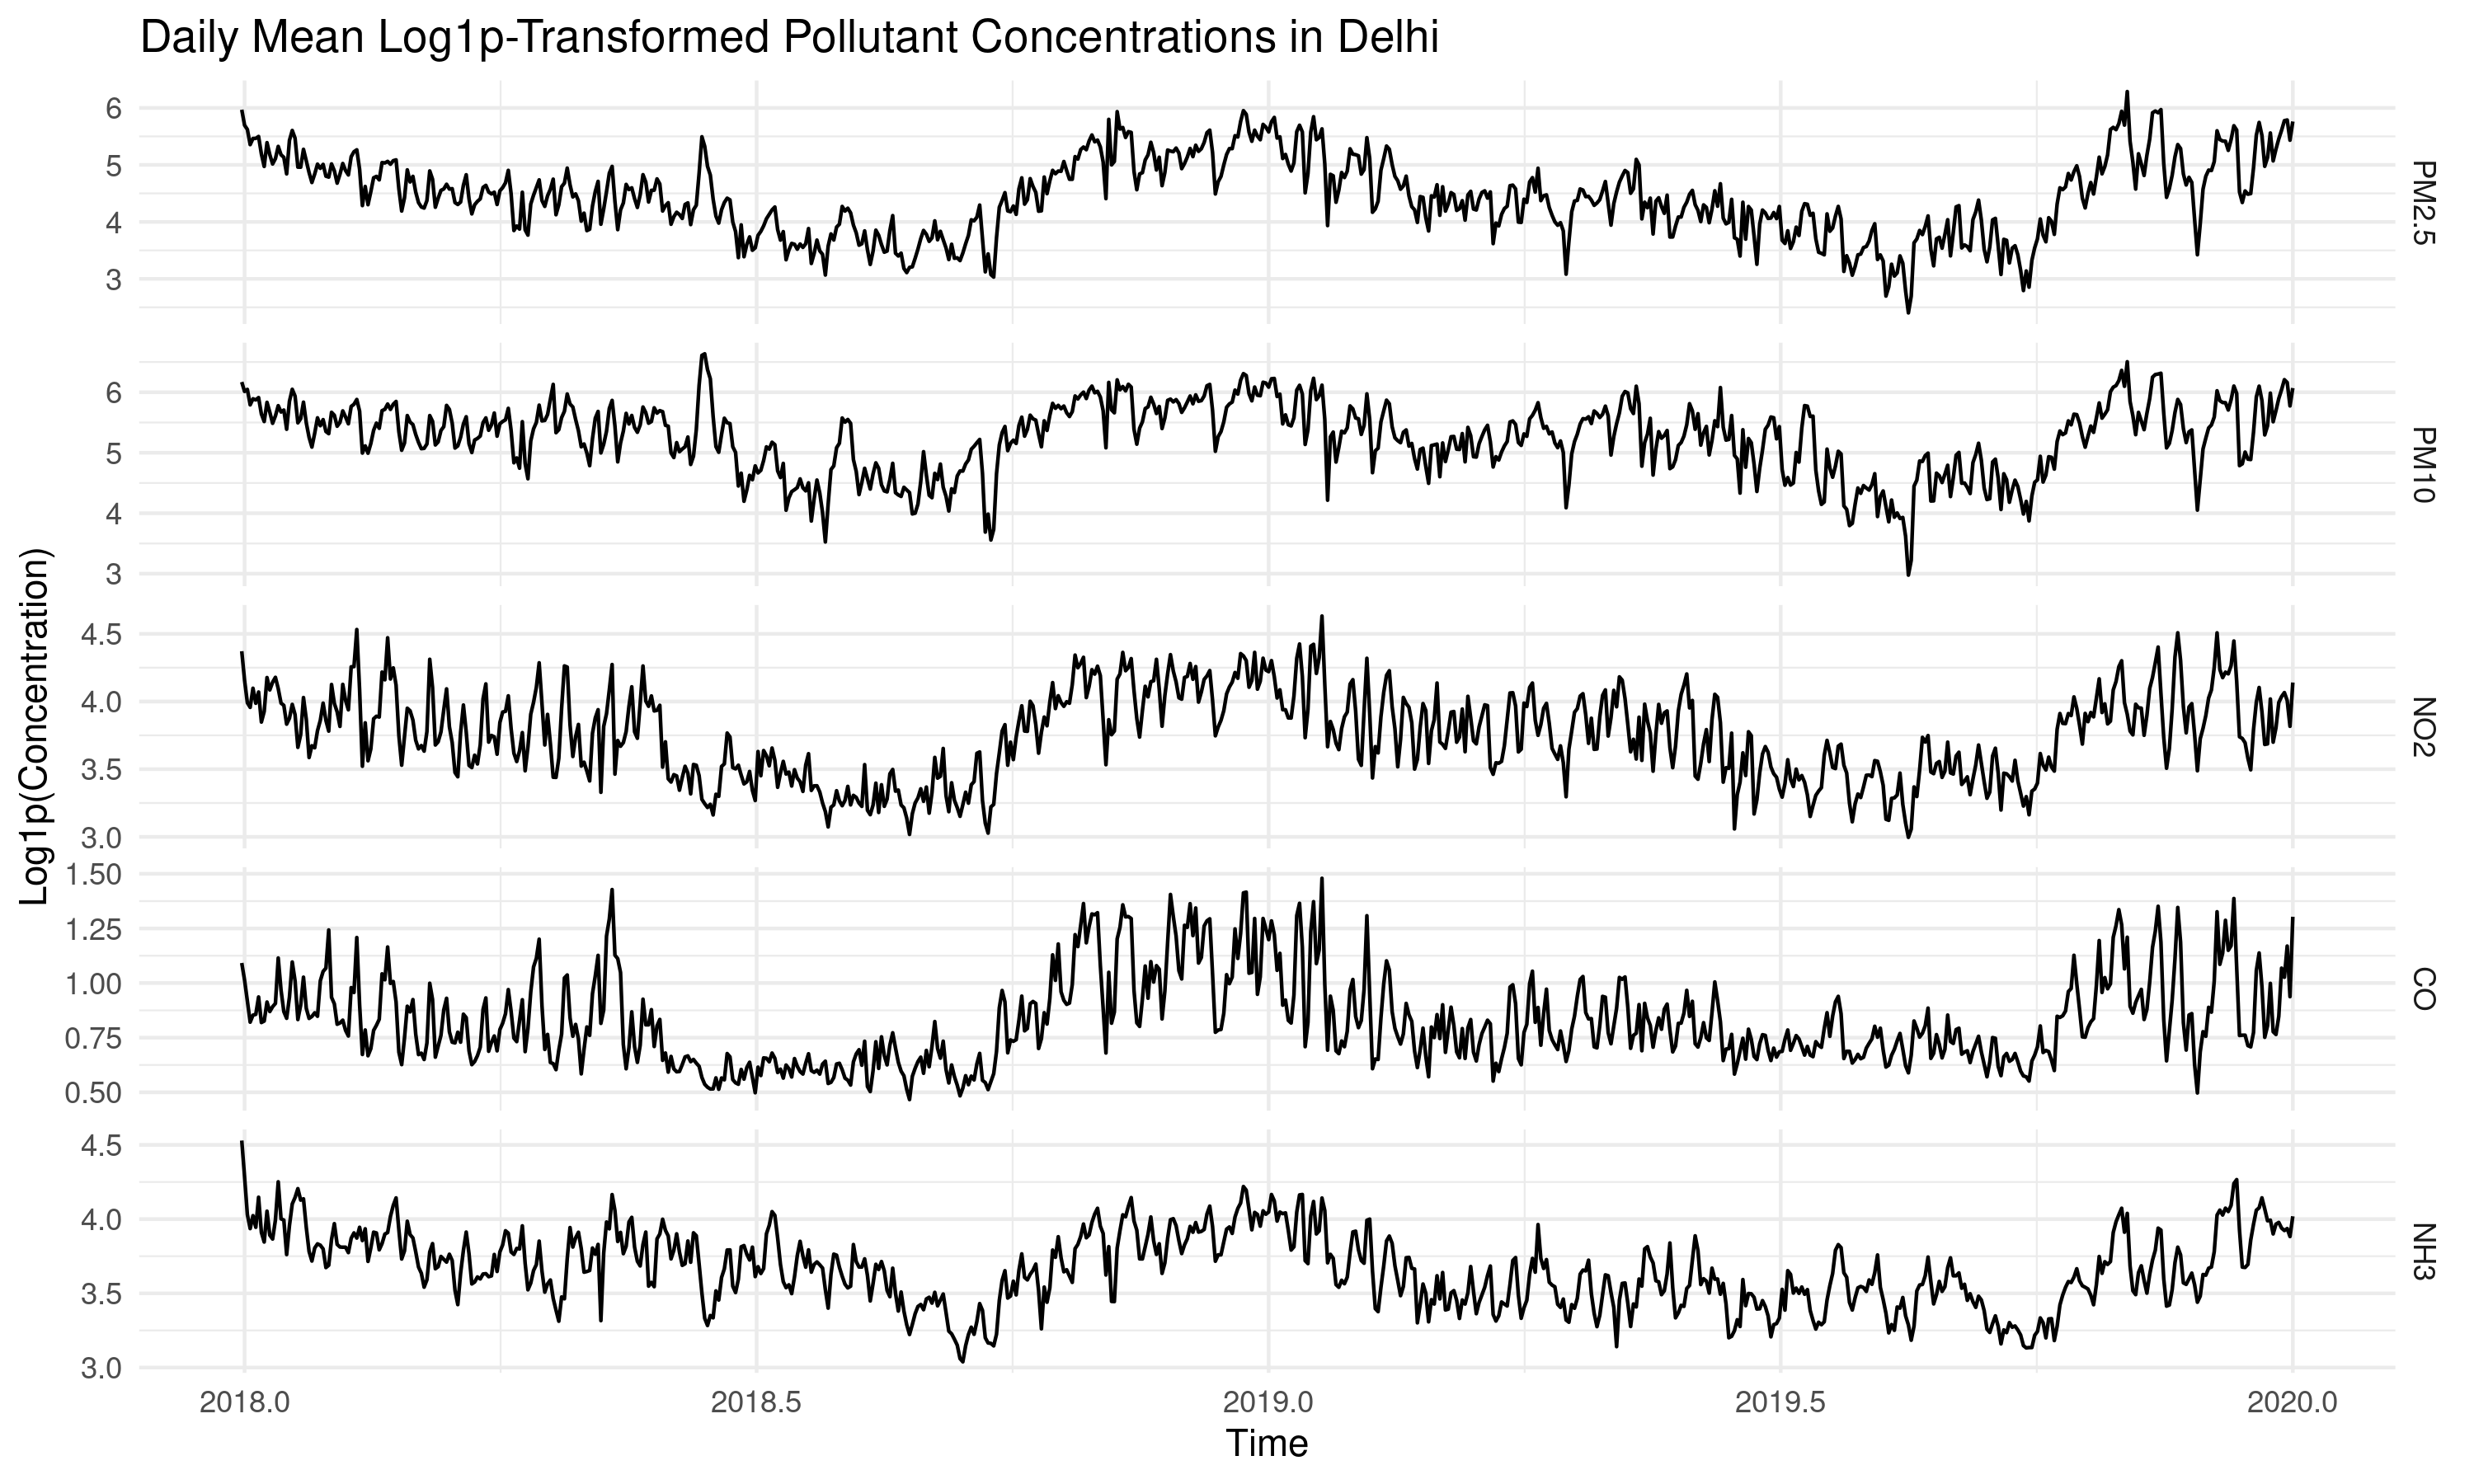
\includegraphics[width=\linewidth]{../analysis/assets/daily_ts_delhi.png}
                \caption*{Daily Log1p-Transformed Pollutants.}
            \end{figure}
        \end{column}
        \begin{column}{0.5\textwidth}
            \textbf{Correlation Matrix:}
            \begin{figure}
                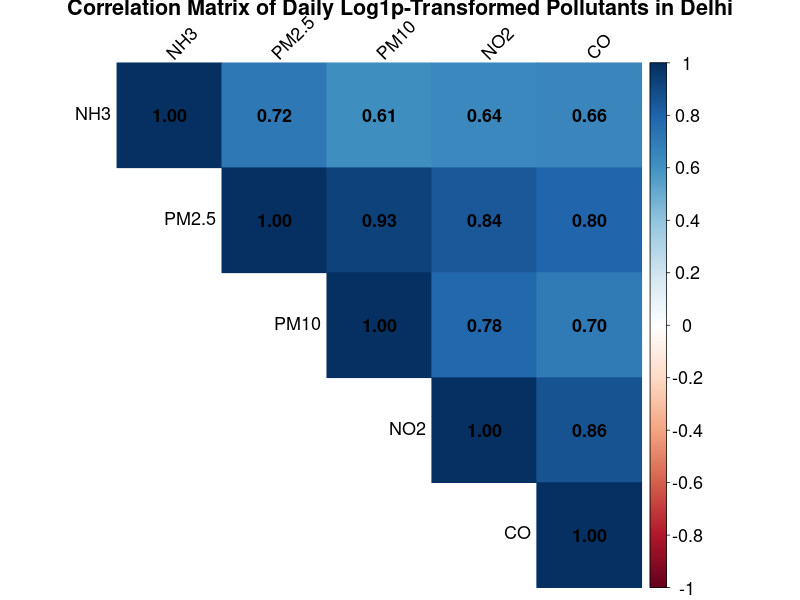
\includegraphics[width=0.9\linewidth]{../analysis/assets/corrplot_delhi.png}
                \caption*{Correlations (Log1p-Transformed).}
            \end{figure}
        \end{column}
    \end{columns}
    \footnotesize Note: Strong interdependencies are evident, motivating multivariate analysis.
\end{frame}

%----------------------------------------------------------------------------------------
\begin{frame}
    \frametitle{Stationarity Testing & Model Choices}
    \begin{itemize}
        \item \textbf{Stationarity Testing:} Augmented Dickey-Fuller (ADF) test on log1p-transformed daily series.
            \begin{center}
            \footnotesize
            \begin{tabular}{lcc}
                \toprule
                Pollutant & Test Statistic & Stationary (p $<$ 0.01) \\
                \midrule
                $PM_{2.5}$ & -5.874 & TRUE \\
                $PM_{10}$  & -7.268 & TRUE \\
                $NO_2$     & -7.986 & TRUE \\
                CO         & -8.681 & TRUE \\
                $NH_3$     & -7.559 & TRUE \\
                \bottomrule
            \end{tabular}
            \end{center}
            \vspace{0.2cm}
            \rightarrow All series are I(0), allowing direct VAR/VARMA application.

        \item \textbf{Vector Autoregression (VAR) Model:}
            $$ Y_t = c + A_1 Y_{t-1} + \dots + A_p Y_{t-p} + \epsilon_t $$
            Optimal lag $p$ via AIC (\texttt{VARselect}). Estimated via \texttt{vars} package.

        \item \textbf{Vector Autoregressive Moving Average (VARMA) Model:}
            $$ Y_t = A_1 Y_{t-1} + \dots + A_p Y_{t-p} + B_1 \epsilon_{t-1} + \dots + B_q \epsilon_{t-q} + \epsilon_t $$
            Estimated via \texttt{MTS} package. VARMA(1,1) explored.
    \end{itemize}
\end{frame}

%----------------------------------------------------------------------------------------
\section{Results and Discussion}
%----------------------------------------------------------------------------------------
\begin{frame}
    \frametitle{VAR(4) Model Analysis: Lag Selection & Causality}
    \begin{itemize}
        \item \textbf{Lag Order Selection for VAR:}
            \begin{itemize}
                \item AIC and FPE suggested $p=4$. HQ suggested $p=2$, SC suggested $p=1$.
                \item \textbf{VAR(4) model selected} based on AIC.
                \item Model stable (all roots of characteristic polynomial $<1$). High $R^2$ values (0.70-0.84).
            \end{itemize}
        \item \textbf{Granger Causality (from VAR(4) model):}
            \begin{center}
            \footnotesize
            \begin{tabular}{lc}
                \toprule
                Causality Direction & $p$-value \\
                \midrule
                $PM_{2.5} \rightarrow$ Others & $4.80 \times 10^{-5}$ *** \\
                $PM_{10} \rightarrow$ Others & $9.81 \times 10^{-4}$ *** \\
                $NO_{2} \rightarrow$ Others & $0.0327$ * \\
                CO $\rightarrow$ Others & $0.174$ \\
                $NH_{3} \rightarrow$ Others & $8.56 \times 10^{-7}$ *** \\
                \bottomrule
            \end{tabular}
            \end{center}
            \vspace{0.2cm}
            \rightarrow Significant predictive relationships, especially from $PM_{2.5}$ and $NH_3$.
    \end{itemize}
\end{frame}

%----------------------------------------------------------------------------------------
\begin{frame}
    \frametitle{VAR(4) Analysis: Impulse Response Functions (IRFs)}
    \begin{itemize}
        \item IRFs trace the effect of a one-standard-deviation shock in one variable on others.
        \item Example: Response of other pollutants to a shock in $NO_2$.
    \end{itemize}
    \begin{figure}
        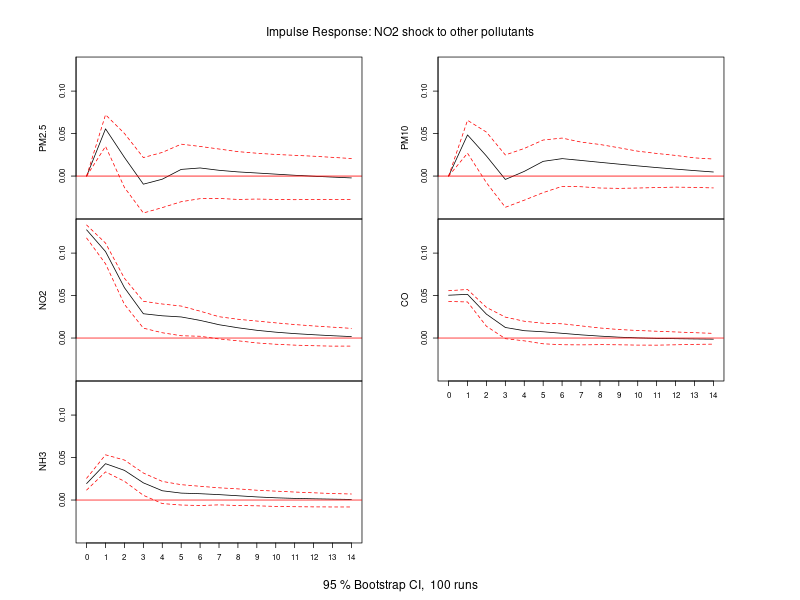
\includegraphics[width=0.9\linewidth]{../analysis/assets/irf_no2_others.png}
        \caption{Impulse Response to 1 SD Shock in $NO_2$ (VAR(4) model, Delhi daily data). Dashed lines: 95\% CI.}
        \label{fig:irf_no2_others_pres}
    \end{figure}
    \begin{itemize}
        \item \footnotesize A positive $NO_2$ shock leads to immediate positive responses in CO and $NH_3$ (lasting ~3 days).
        \item \footnotesize Positive responses in $PM_{2.5}$ and $PM_{10}$ appear after a 1-day lag. Responses die out over time.
    \end{itemize}
\end{frame}

%----------------------------------------------------------------------------------------
\begin{frame}
    \frametitle{VAR(4) Analysis: Forecast Error Variance Decomposition (FEVD)}
    \begin{itemize}
        \item FEVD shows the proportion of forecast error variance of each variable attributable to its own shocks versus shocks from other variables.
    \end{itemize}
    \begin{figure}
        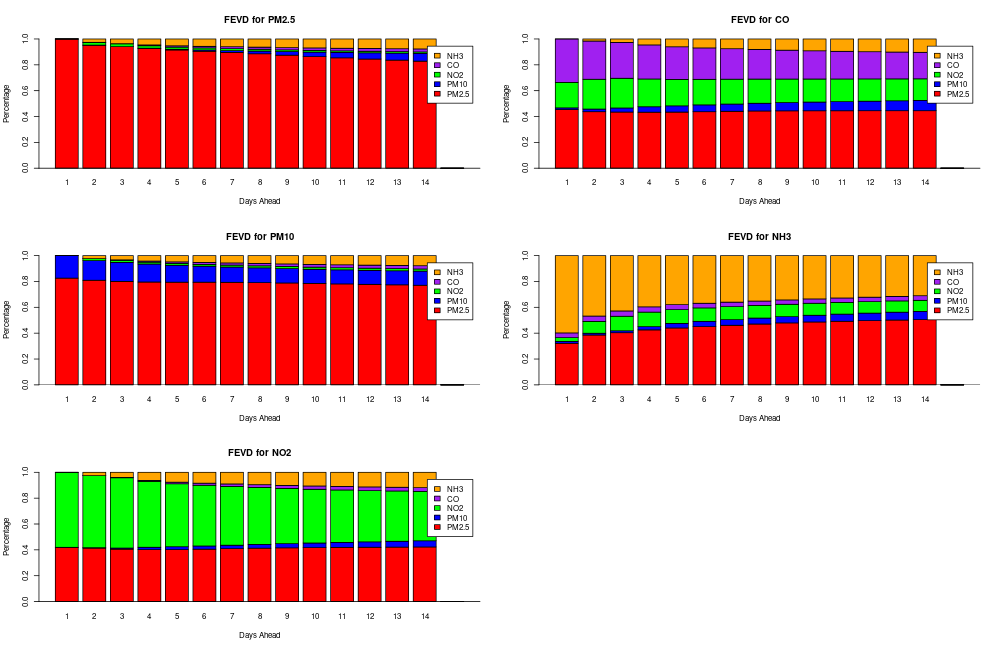
\includegraphics[width=0.9\linewidth]{../analysis/assets/fevd_delhi.png}
        \caption{FEVD of Daily Log1p-Transformed Pollutants (VAR(4) Model, 10-day horizon).}
        \label{fig:fevd_delhi_pres}
    \end{figure}
    \begin{itemize}
        \item \footnotesize Large portion of forecast error variance for most pollutants is explained by their own shocks or by $PM_{2.5}$ shocks.
        \item \footnotesize Example: $NO_2$ shocks explain ~17.8\% of $CO$'s forecast error variance at a 10-day horizon.
    \end{itemize}
\end{frame}

%----------------------------------------------------------------------------------------
\begin{frame}
    \frametitle{Forecasting Evaluation: VAR(4) vs. VARMA(1,1)}
    \begin{itemize}
        \item \textbf{Setup:}
            \begin{itemize}
                \item Data split: Training (first 718 days), Test (last 14 days).
                \item Forecast horizon: 14 days ahead.
                \item Metric: Root Mean Squared Error (RMSE) on log1p-transformed scale.
            \end{itemize}
        \item \textbf{RMSE Comparison on Test Set:}
            \begin{center}
            \footnotesize
            \begin{tabular}{lccccc}
                \toprule
                Model      & $PM_{2.5}$ & $PM_{10}$ & $NO_2$ & $CO$  & $NH_3$ \\
                \midrule
                VAR(4)     & 0.721      & 0.543     & 0.179  & 0.202 & 0.150  \\
                \textbf{VARMA(1,1)} & \textbf{0.605} & \textbf{0.446} & \textbf{0.169} & \textbf{0.189} & \textbf{0.142} \\
                \bottomrule
            \end{tabular}
            \end{center}
            \vspace{0.2cm}
            \rightarrow VARMA(1,1) showed lower RMSE for all five pollutants, suggesting better point forecast accuracy for this dataset and horizon.
    \end{itemize}
\end{frame}

%----------------------------------------------------------------------------------------
\begin{frame}
    \frametitle{Example: VAR(4) Forecasts for Delhi Pollutants}
    \begin{figure}
        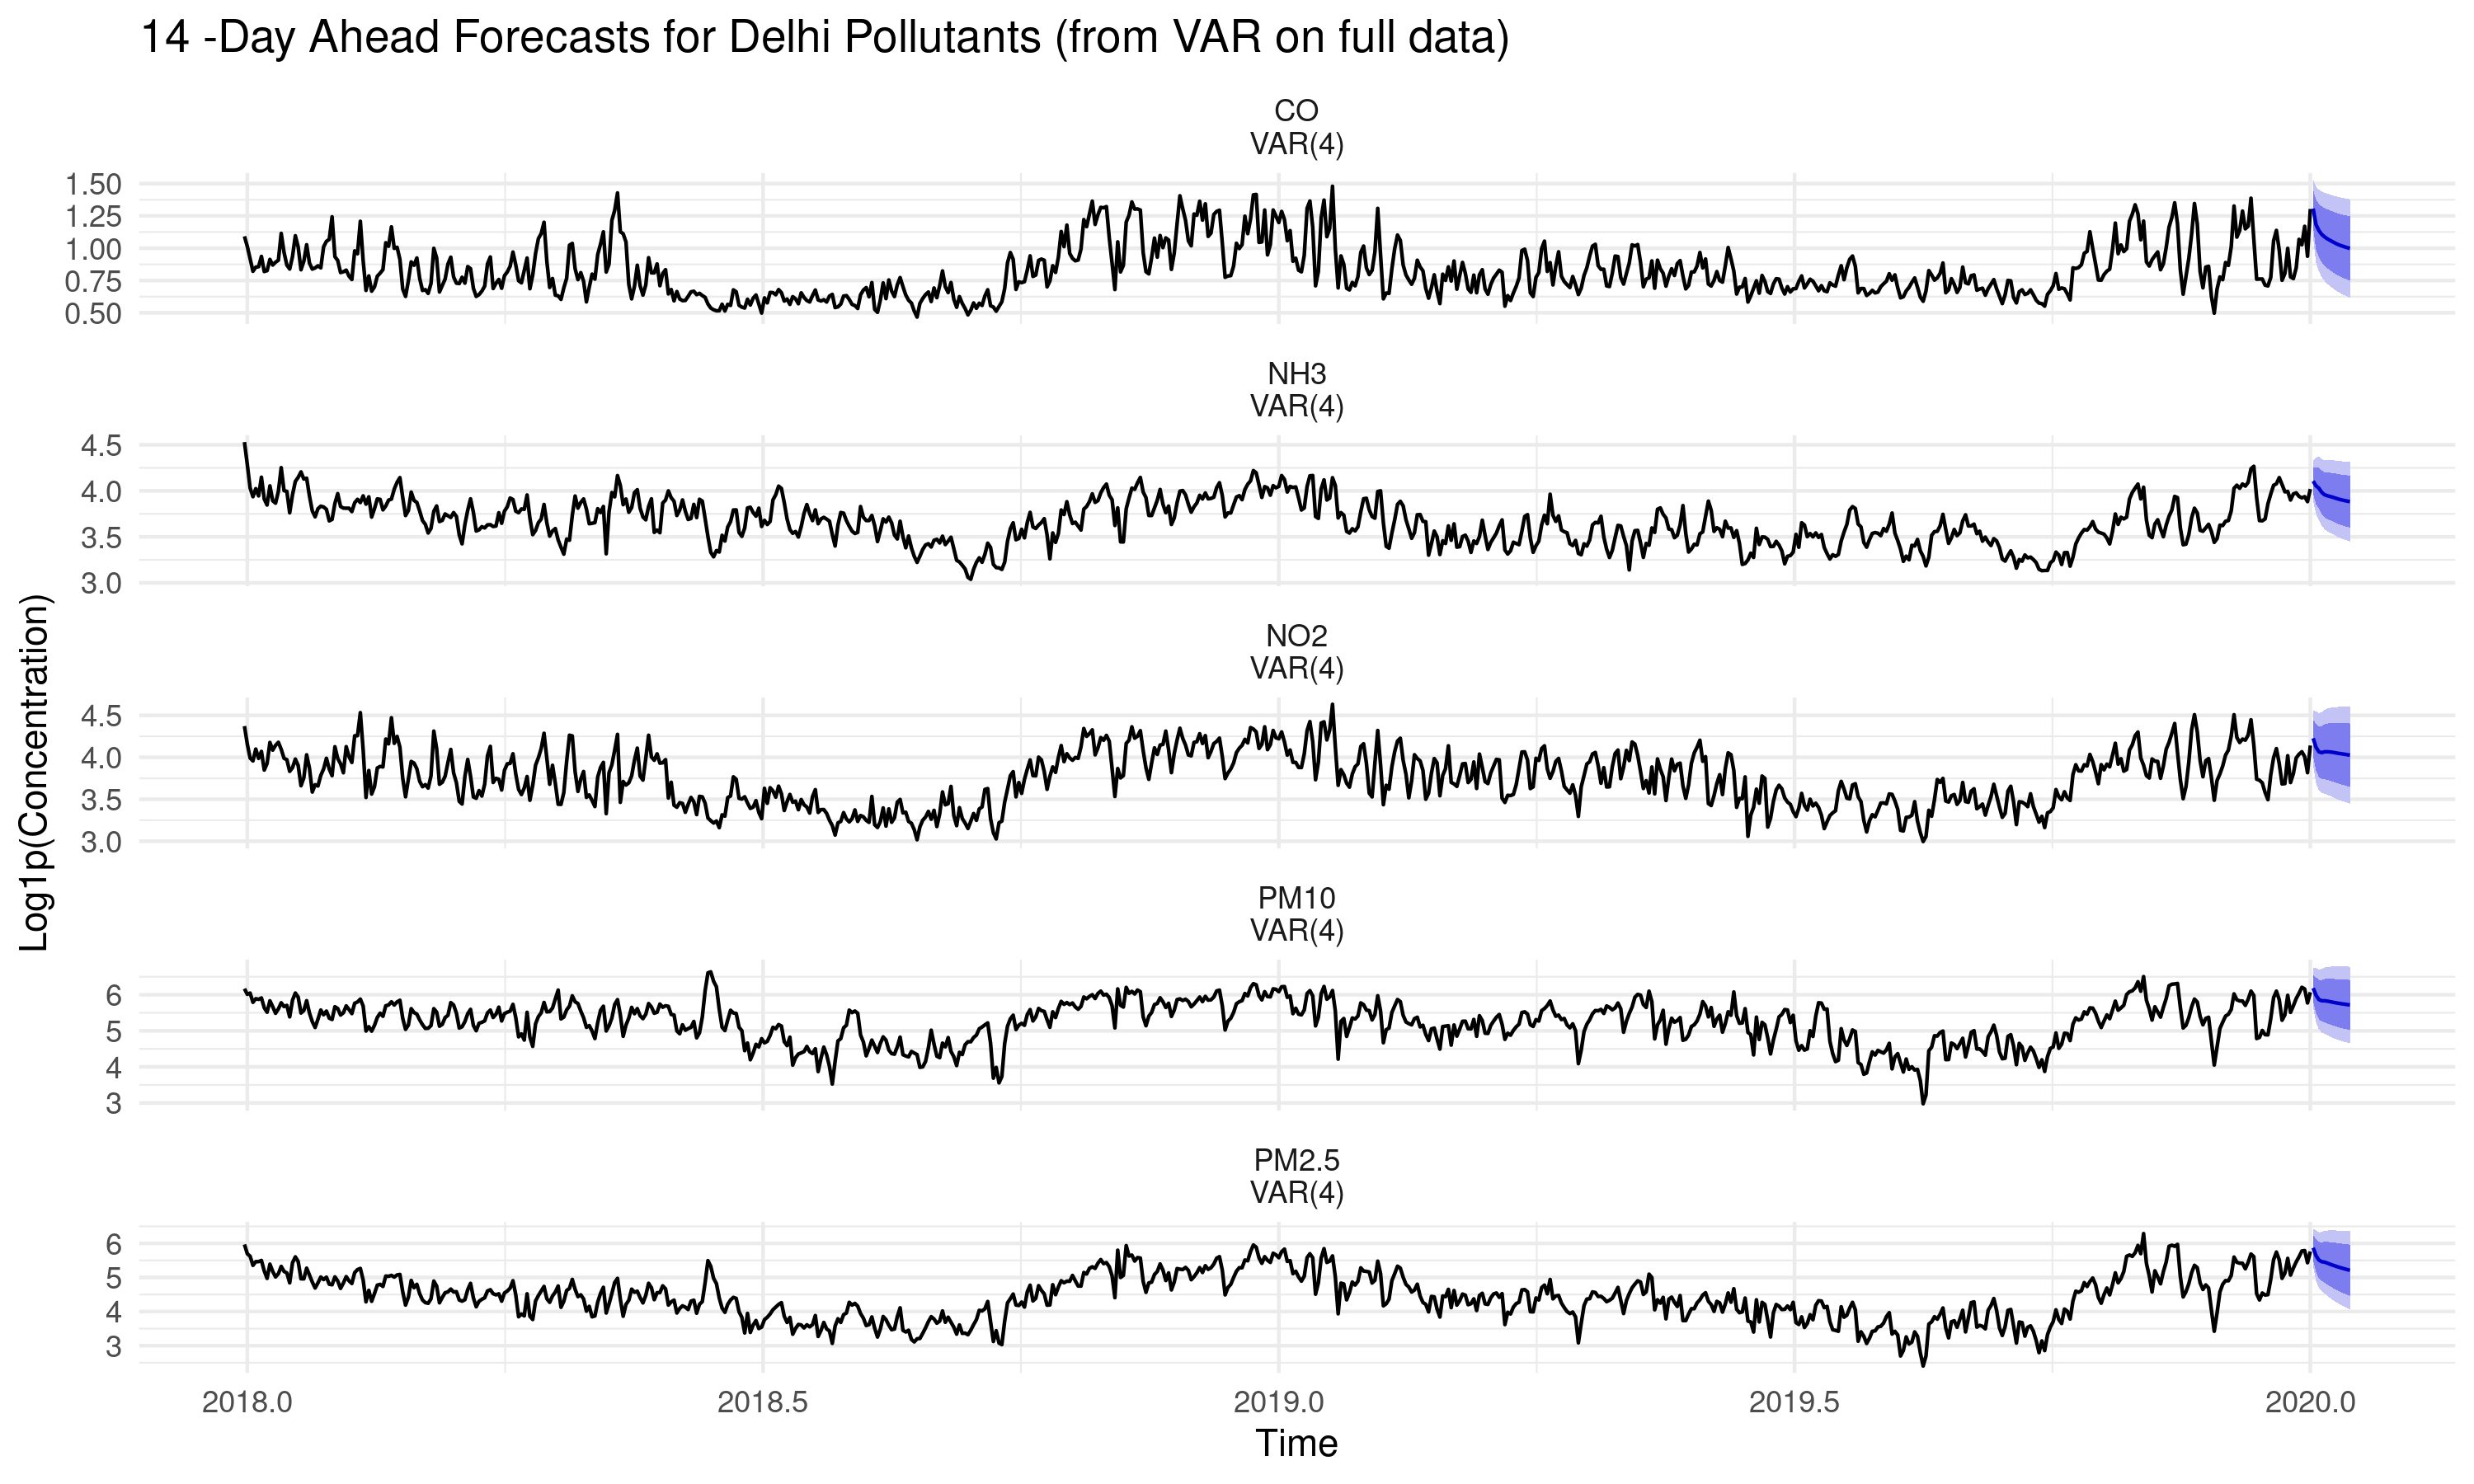
\includegraphics[width=\linewidth]{../analysis/assets/var_forecast_delhi.png}
        \caption{14-Day Ahead Forecasts from VAR(4) Model (Trained on Full Daily Data). Point forecasts with 80\% and 95\% CIs.}
        \label{fig:var_forecast_delhi_pres}
    \end{figure}
    \begin{itemize}
        \item \footnotesize Forecasts tend to revert to the mean, with widening confidence intervals as the horizon increases.
    \end{itemize}
\end{frame}

%----------------------------------------------------------------------------------------
\section{Conclusion and Future Work}
%----------------------------------------------------------------------------------------
\begin{frame}
    \frametitle{Conclusion}
    \begin{itemize}
        \item Successfully applied VAR and VARMA models to analyze multivariate dynamics of 5 key air pollutants in Delhi (2018-2019).
        \item Daily log1p-transformed pollutant series were found to be stationary I(0).
        \item VAR(4) model revealed:
            \begin{itemize}
                \item Significant Granger causalities (e.g., $PM_{2.5}$, $NH_3$ influencing others).
                \item Dynamic interactions via IRFs (e.g., $NO_2$ shocks affect other pollutants).
                \item FEVD showed importance of own shocks and $PM_{2.5}$ in forecast error variance.
            \end{itemize}
        \item For 14-day ahead forecasting, VARMA(1,1) outperformed VAR(4) in terms of RMSE.
        \item The study highlights the interconnected nature of air pollution and the utility of multivariate models.
    \end{itemize}
\end{frame}

%----------------------------------------------------------------------------------------
\begin{frame}
    \frametitle{Limitations and Future Work}
    \begin{block}{Limitations}
        \begin{itemize}
            \item Focus on a single city (Delhi).
            \item Limited set of pollutants.
            \item Use of linear models (VAR/VARMA).
            \item Daily aggregation might mask hourly dynamics.
            \item VARMA order selection was illustrative (1,1), not exhaustive.
        \end{itemize}
    \end{block}
    \vspace{0.5cm}
    \begin{block}{Future Work}
        \begin{itemize}
            \item Extend to multiple cities (spatial dependencies).
            \item Incorporate exogenous variables (e.g., meteorological data).
            \item Explore non-linear multivariate models.
            \item Investigate seasonal decomposition methods prior to modeling.
            \item Use more granular (hourly) data, if computationally feasible.
            \item Advanced VARMA order selection and diagnostics.
        \end{itemize}
    \end{block}
\end{frame}

%----------------------------------------------------------------------------------------
\section*{References}
%----------------------------------------------------------------------------------------
\begin{frame}[allowframebreaks] % allowframebreaks allows the content to span multiple slides if needed
    \frametitle{References}
    \footnotesize
    \begin{thebibliography}{99} % Use 99 to allow for double digits if many references
        \bibitem{aladag2021}
        Aladağ, E. (2021). \textit{Forecasting of Particulate Matter with a Hybrid ARIMA Model Based on Wavelet Transformation and Seasonal Adjustment}. Urban Climate.
        
        \bibitem{hajmohammadi2021}
        Hajmohammadi, H. and Heydecker, B. (2021). \textit{Multivariate time series modelling for urban air quality}. Urban Climate.
        
        \bibitem{sethi2020}
        Sethi, J.K. and Mittal, M. (2020). \textit{Analysis of Air Quality using Univariate and Multivariate Time Series Models}. IEEE Confluence.
        
        \bibitem{RCoreTeam2025}
        R Core Team (2025). \textit{R: A Language and Environment for Statistical Computing}. R Foundation for Statistical Computing, Vienna, Austria.
        
        \bibitem{dplyr}
        Wickham, H., et al. (2023). \textit{dplyr: A Grammar of Data Manipulation}. R package version 1.1.4.
        
        \bibitem{ggplot2}
        Wickham, H. (2016). \textit{ggplot2: Elegant Graphics for Data Analysis}. Springer-Verlag New York.
        
        \break % Manual break if needed, or let allowframebreaks handle it

        \bibitem{tidyr}
        Wickham, H., et al. (2024). \textit{tidyr: Tidy Messy Data}. R package version 1.3.1.
        
        \bibitem{forecast}
        Hyndman, R., et al. (2025). \textit{forecast: Forecasting functions for time series and linear models}. R package version 8.24.0.
        
        \bibitem{urca}
        Pfaff, B. (2008). \textit{Analysis of Integrated and Cointegrated Time Series with R}. Second Edition. Springer, New York.
        
        \bibitem{vars}
        Pfaff, B. (2008). \textit{VAR, SVAR and SVEC Models: Implementation Within R Package vars}. Journal of Statistical Software.
        
        \bibitem{MTS}
        Tsay, R. S., et al. (2022). \textit{MTS: All-Purpose Toolkit for Analyzing Multivariate Time Series (MTS) and Estimating Multivariate Volatility Models}. R package version 1.2.1.
    \end{thebibliography}
\end{frame}

%----------------------------------------------------------------------------------------
% Q&A SLIDE
%----------------------------------------------------------------------------------------
\begin{frame}{Thank You!}
	\begin{center}
		\Huge Thank you for your attention!
	\end{center}
\end{frame}

%----------------------------------------------------------------------------------------

\end{document}